\documentclass[11pt,parskip,abstracton,notitlepage]{scrartcl}

\makeatletter
\DeclareOldFontCommand{\rm}{\normalfont\rmfamily}{\mathrm}
\DeclareOldFontCommand{\sf}{\normalfont\sffamily}{\mathsf}
\DeclareOldFontCommand{\tt}{\normalfont\ttfamily}{\mathtt}
\DeclareOldFontCommand{\bf}{\normalfont\bfseries}{\mathbf}
\DeclareOldFontCommand{\it}{\normalfont\itshape}{\mathit}
\DeclareOldFontCommand{\sl}{\normalfont\slshape}{\@nomath\sl}
\DeclareOldFontCommand{\sc}{\normalfont\scshape}{\@nomath\sc}
\makeatother

\usepackage{amssymb, amsmath, amsthm, graphics, graphicx, longtable, setspace, makeidx, subfig, marvosym, microtype, booktabs, tabularx,authblk, lipsum, siunitx, lmodern, makecell, rotating, pdflscape,fullpage, dcolumn}

\usepackage{tikz}
\usetikzlibrary{arrows} 
\usetikzlibrary{backgrounds}
\usetikzlibrary{fit}
\usepackage{animate}
\usepackage{extarrows}
\usepackage{pgf}
\usepackage{pgfplots} 
\usepackage{relsize}
\usepackage[margin=10pt,font=small,labelfont=bf,labelsep=endash]{caption}

\usepackage[style= authoryear, backend=bibtex,natbib=true, firstinits=true, uniquename=true,backref=false,doi=false,isbn=false,url=false,maxnames=2, maxbibnames=10, dashed =true]{biblatex}
\renewcommand*{\compcitedelim}{\addsemicolon\space}
\renewbibmacro{in:}{}
\setlength\bibhang{20pt}
\bibliography{ref}
\AtEveryBibitem{%
	\clearfield{day}%
	\clearfield{month}%
	\clearfield{endday}%
	\clearfield{endmonth}%
}
\doublespacing

\newtheorem{proposition}{Proposition}
\newtheorem{definition}{Definition}
\newtheorem{assumption}{Assumption}
\newtheorem{lemma}{Lemma}
\newenvironment{MYenumerate}{\renewcommand{\labelenumi}{(\roman{enumi})}\renewcommand{\labelenumii}{\arabic{enumii}.}
\begin{enumerate}}{\end{enumerate}}
\renewcommand{\baselinestretch}{1.3}

\usepackage[pdftex,colorlinks=true,citecolor=red,urlcolor=magenta,pdfstartview=FitH]{hyperref}
        		\pdfcompresslevel=9
      \hypersetup{pdftitle={On spatial dependence in stochastic frontier models with an application to European regional economic performance},
		   		pdfauthor={Thomas de Graaff},
		   		pdfsubject={},
		   		pdfkeywords={},
		   		pdffitwindow=true} 
    

\begin{document}
%\input{SSF-concordance}

\title{\bfseries On spatial dependence in stochastic frontier models with an application to European regional economic performance}
\author{Thomas de Graaff $^{a}$\thanks{Corresponding author. Tel +31 (0)20
    5986092. Email: \href{t.de.graaff@vu.nl}{t.de.graaff@vu.nl}. Paper, code and presentation can be found
    on
    \href{https://github.com/Thdegraaff/SpatFrontier}{https://github.com/Thdegraaff/SpatFrontier}. A specific package website can be found on \href{http://www.thomasdegraaff.nl/SpatFrontier/}{http://www.thomasdegraaff.nl/SpatFrontier/}, but is at the moment still under heavy development. This paper is prepared for the 17$^{th}$ workshop on spatial econometrics and statistics in Dijon 2018. The author would like to thank Ferdinand Paraguas, Raymond Florax and Henri de Groot for useful comments on earlier versions of the paper.} \bigskip \ \ \ 
\and 
{\small {$^{a}$ \emph{Department of Spatial Economics, Faculty of Economics and Business Adminstration}}} \\
{\small {\emph{VU University, Amsterdam, The Netherlands}}} \bigskip \\
}

\date{\today}
\maketitle
\clearpage

\begin{abstract}
\noindent In this paper I argue that the diffusion of technology across regions
is spatially restricted in nature. Thus, that a region's technical
efficiency---its relative economic performance given its endowments---may depend
more on regions nearby than on a `global' level of technology. We estimate these
spatially related technical efficiencies by using a spatial stochastic frontier
model, most notably we control for spatially correlated errors. Specifically, my
contribution is threefoldt.  Using a relatively straightforward approach this
study shows how to combine a spatial error structure with a stochastic frontier
model that is (\emph{i}) straightforward to estimate, (\emph{ii}) able to
separate spatial dependence in the error term and technical efficiencies, and
(\emph{iii}) produce consistent estimates. So, I am able to make a distinction between technical efficiencies related to the use of a region's endowments and those related to spatial dependence: in other words, between a region's absolute and a region's relative location. Using newly constructed regional data on European regional output, labor levels and especially capital level, our results indicate that European technical efficiencies are indeed very much spatially related.
\noindent 
\newline
\newline
{\small \textbf{Keywords:} Spatial dependence, stochastic frontiers, skew-normal distribution \newline
\textbf{JEL-classification:} R1, R3}
\end{abstract}
\thispagestyle{empty}

\section{Introduction}
%
One of the most distinct features of European regions is that they differ widely in their economic performance, even when controlling for the number of inhabitants. Obviously, countries differ in terms of institutions, culture, stability, and so forth, which determine for a large part the international differences in economic performance. However, wealth and income are sometimes even more dispersed \emph{within} countries than across countries. To illustrate this, Figure \ref{fig:gdppc} shows the dispersion of relative regional GDP per capital across European countries.

\begin{figure}[h]
	\center
	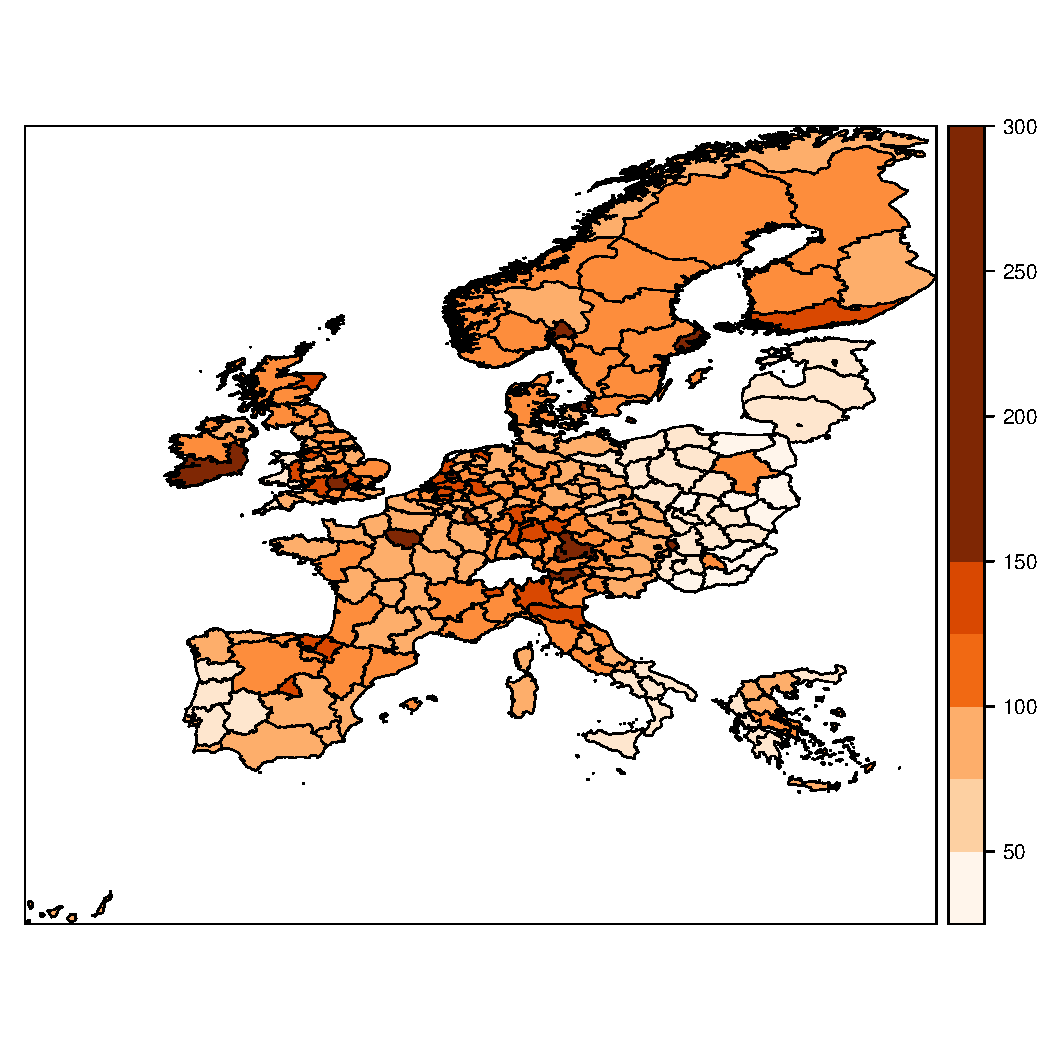
\includegraphics[width=0.8\textwidth]{fig/gdppc}
	\caption{GDP per capita across Europe in 2007---EU27 = 100 (source: cambridge econometrics database}
	\label{fig:gdppc}
\end{figure}

Obviously, European wealth is accumulated within large metropolitan areas (most notably---the capital cities) such as Paris, London, Luxembourg, Oslo and Stockholm. However, apart from this, large differences are present as well between subnational regions. The most well-known example is the North-South division within Italy, but these differences can as well be noticed within almost all countries in Europe. Most notable examples are Spain (North-South division as well), France (with a relatively poorer central area), the UK (where the periphery seems to be much poorer), and Germany (with the former division between East and West). Thus, some regions within countries are significantly more successful than others---even when faced with similar national institutions. 

What makes regions successful? This is probably the most crucial and complex research question for both regional policymakers and regional scientists to answer. Regional policy makers would like to create policies aimed to steer regions to success, regional scientists are especially interested in the (nature of the) determinants that drive this success. At the heart, this research question deals with the absolute and relative location advantages of regions.\footnote{There is a large debate about the drivers of economic success, both on a national and a regional level. Some scientist favor the proposition that regions prosper because of historical events and the associated path-dependencies \citep[e.g.,][]{LANDES1998}, while others emphasize absolute \citep[e.g.][]{diamond1998guns} and relative \citep[e.g.,][]{FUJITA1999} locational advantages. Obviously, these different drivers require different policy instruments---if any at all.}

A strongly related research question deals with the exact nature of economic performance. How to define economic performance and how to measure it is still subject to an ongoing debate. Already numerous studies have conducted with the purpose of benchmarking cities, regions and the like. Usually, these studies are not based on any behavioral or economic structure. Further, although sometimes population size is taken into account, the level of other initial endowments is usually neglected. Ideally, the latter should be taken into account in the question whether regions are successful \emph{given} their initial situation. In the economics literature this can be reflected in the idea of stochastic frontier analysis. Here, firm performance is measured as the technical efficiency in their employment of production factors. The closer the firm's output is relative to the best possible output, the higher the firm's technical efficiency. Analogously, one can consider regions as production units (as is often done) and look at the region's technical efficiency in employing their endowments. As Figure \ref{fig:gdppc} clearly shows, some regions are probably more efficient than others---even within the same country. And this should be reflected when benchmarking those regions. 

The left production isoquant in Figure \ref{fig:isoquants} shows how a region's technical efficiency can be measured. Denote $y$ as the \emph{given} maximum attainable production a region can get using the production factors $x_1$ and $x_2$. Regions $A_1, A_2, A_3, B_1, B_2$ and $B_3$ are all producing inefficiently. With the same amount of production factors $x_1$ and $x_2$ that theoretically enable them to produce $y$, they produce on average $\hat{y}$. The distance between $Y$ and $\hat{y}$ is then a measure for the average efficiency. More precisely, efficiency is defined as the ratio $\vec{\hat{y}}/\vec{y}$ where  $\vec{y}$ is the length of the line between the origin and $y$. As a result, technical efficiencies must be smaller than 1. 

\begin{figure}[t]
\tikzstyle{backgroundB}=[circle, fill=blue!10,inner sep=0.5cm]
\tikzstyle{backgroundA}=[circle, fill=red!10,inner sep=0.5cm]
\begin{center}

\begin{tikzpicture}[
		scale = 1.2,
		frontier/.style={black,thick},
		axis/.style={very thick , ->, >=stealth', line join=miter},
		region/.style={circle, fill=black, minimum size=4pt, inner sep=0pt, outer sep=-1pt},
		]

	\draw[axis,<->] (5,0) node(xline)[below] {$x_1$} - | 
				(0,5) node(yline)[left]{$x_2$};
	\draw[frontier] (1.5,5) to[out=270,in=180] (5,1.5)node[right] {$y$}  ;
	\node (A1) [region,label=above:$A_1$] at (1,4.2) {};
	\node (A2) [region,label=above:$A_2$] at (2,2.5) {};
	\node (A3) [region,label=above:$A_3$] at (3.5,1.2) {};
	\draw[frontier, black!80, dashed] (0.5,5) to[out=270,in=180] (5,0.5) node[right] {$\hat{y}$} ;
	\node (B1) [region,label=above:$B_1$] at (0.5,2.9) {};
	\node (B2) [region,label=above:$B_2$] at (1.4,1.4) {};
	\node (B3) [region,label=above:$B_3$] at (2.75,0.85) {};
	\draw[->, black!50, >=stealth'] (0,0) -- (3.05,2.05);	
	\draw[->, very thick, black, >=stealth'] (2.2,1.48) -- (3.05,2.05)
		node[sloped, above, midway] {$TE$};		
			
	\draw[axis,<->] (11,0) node(xline)[below] {$x_1$} - |
				(6,5) node(yline)[left]{$x_2$};
	\draw[frontier] (7.5,5) to[out=270,in=180]  (11,1.5) node[right] {$y$};
	\node (A11) [region,label=above:$A_1$] at (7,4.2) {};
	\node (A21) [region,label=above:$A_2$] at (8,2.5) {};
	\node (A31) [region,label=below:$A_3$] at (9.5,1.2) {};	
	\draw[frontier, black!30, dashed] (6.5,5) to[out=270,in=180] (11,0.5) node[right] {$\hat{y}$};
	\draw[frontier, red!80, dashed] (7,5) to[out=270,in=180] (11,0.75) node[right] {$\hat{y_A}$};
	\draw[frontier, blue!80, dashed] (6.1,5) to[out=270,in=180] (11,0.2) node[right] {$\hat{y_B}$};
	\node (B11) [region,label=above:$B_1$] at (6.5,2.9) {};
	\node (B21) [region,label=above:$B_2$] at (7.4,1.4) {};
	\node (B31) [region,label=above:$B_3$] at (8.75,0.85) {};		
	\draw[->, black!30, >=stealth'] (6,0) -- (9.05,2.05);	
	\draw[->, very thick, black!30, >=stealth'] (8.2,1.48) -- (9.05,2.05)
		node[sloped, above, midway] {$TE$};
	\draw[->, blue!30, >=stealth'] (6,0) -- (8,3.1);			
	\draw[->, very thick, blue!80, >=stealth'] (7.24,1.9) -- (8,3.1)
		node[sloped, above, midway] {$TE_B$};
	\draw[->, red!30, >=stealth'] (6,0) -- (10.2,1.6);	
	\draw[->, very thick, red!80, >=stealth'] (9.18,1.22) -- (10.18,1.61)
		node[sloped, above, midway] {$TE_A$};
		
	\begin{pgfonlayer}{background}
		\node[backgroundB, fit =(B11)]{};	
		\node[backgroundB, fit =(B21)]{};	
		\node[backgroundB, fit =(B31)]{};					
		\node[backgroundA, fit =(A11)]{};	
		\node[backgroundA, fit =(A21)]{};	
		\node[backgroundA, fit =(A31)]{};		
	\end{pgfonlayer}
\end{tikzpicture}
\end{center}
\caption{Production possibility frontiers in a standard (left) and a spatial structure (right).}
\label{fig:isoquants}
\end{figure}


There is already a sizeable literature dealing with benchmarking regions using regional technical efficiencies.\footnote{See, amongst others, \citet{BROCK1999, puig2001technical, puig2008some, ALVAREZ2007}.} This literature usually deals with the relative (sectoral) performance of regions and this is the approach this paper takes as well. The production factors are then usually constituted of the aggregates of various forms of labour (high skilled and low skilled) and capital (both physical and human) within a region. 

Estimation of technical efficiencies may, however, be biased in the presence of spatial dependence or unobserved spatial heterogeneity amongst regions. Namely, when one assumes that only neighboring regions benefit from other regions' technological knowledge through the traditional Marshallian channels of shared customers and suppliers, shared labor pools or spillover mechanisms (or just through unobserved spatial heterogeneity), then straightforward estimation of technical efficiencies is biased. This can be been in the right production isoquant depicted in Figure \ref{fig:isoquants}. Assume that regions $A_1, A_2$ and$A_3$ belong to country $A$ and regions $B_1, B_2$ and $B_3$ belong to country $B$, then it quite well conceivable because of spatial unobserved heterogeneity or spatial dependence that the technical efficiencies of the regions in country $A$ and $B$ are related. In Figure \ref{fig:isoquants}, region $B_3$ might not produce inefficient at all \emph{given} the fact that neighbouring regions in country $B$ produce even less efficient. This works as well the other way around. Regions very central in a network and surrounded by very efficiently producing regions, have besides a strong economic structure probably a very favourable location as well. In this context, efficiency can be related to advantages related to the \emph{absolute} location while spatial dependence relates to the \emph{relative} location. To control for both the inefficiency in production and the geographical location, we therefore aim to explicitly incorporate a spatial correlation structure in stochastic production frontiers. 

The literature that combines spatial dependence and stochastic production frontiers is, although relatively recent, already very sizable. Most studies employ a parametric approach and the enumeration that follows is definitely not conclusive. One of the first parametric studies was \citet{BARRIOS2010}, who uses an interative backfitting algorithm to find consistent parameter estimates although they do not allow for correlation between the technical efficiency and spatial dependence structure. \citet{PAVLYUK2010} uses as well a parametric approach, but does not report how he estimates consistently both the spatial dependence process and technical efficiencies.  \citet{fusco2013spatial} separate out the error term in a spatial lag structure and technical efficiencies, with an application to the Italian wine sector. \citet{kinfu2015inefficiency} apply a spatial stochastic frontier analysis to maternal care in India. \citet{glass2013productivity} decomposes productivity growth using a spatial autoregressive model, whereafter \citet{glass2016spatial} extends the model itself to a spatial panel setting. Finally, \citet{jiang2017energy} apply a fixed effects stochastic frontier model to energy efficiency in Chinese provinces. In addition, there is a smaller literature that resorts to a Bayesian approach and simulation techniques, i.e. \citet{SCHMIDT2009} and \citet{AREAL2010}.  

A specific criticism that applies to most of these (specifically parametric) studies is that they all consider a univariate error term once the spatial component is accounted for. However, as I will argue below, the error term is by definition multivariate as it is a combination of a normal and truncated normal distribution, where one of them or even both are multivariate due to the spatial correlation structure. 

In contrast this study applies a different multivariate approach firmly rooted in the statistical literature. Using a relatively straightforward approach this study shows how to combine a spatial error structure with a stochastic frontier model that is (\emph{i}) straightforward to estimate, (\emph{ii}) able to separate spatial dependence in the error term and technical efficiencies, and (\emph{iii}) produce consistent estimates. Moreover, I indicate how to incorporate more general spatial lag structures in stochastic frontier models. Estimation of these models, however, require simulation techniques.

The remainder of this paper is structured as follows. The next section
introduces the concept of regional technical efficiencies and discusses some
measurement issues. Consecutively, it treats the modeling (and its associated
estimation) of technical efficiencies in two ways: a mainly econometric and a
more statistical one.\footnote{Actually, both modeling approaches date back to
  one common source: namely, \cite{WEINSTEIN1964}.} The third section deals with
the introduction of spatial dependence in stochastic production frontiers.
Section 4 provides simulation results to indicate the performmance of my
estimation methods vis-\'{a}-vis other estimation methods. Section \ref{sec:Applications} provides an application of spatial stochastic frontier modeling and gives an estimation of the technical efficiencies of European NUTS2 regions in 2010. The last section concludes.
%
\section{Measuring technical inefficiencies}
%
Since the late 70s, economists increasingly recognized that, although having access to the same set of production factors, firms do not necessarily produce the same output---and that there was consequently a need to econometrically correct for that (the seminal papers of this econometric literature are \citet{AIGNER1977} and \citet{MEEUSEN1977}). To explain this variation in output, it was argued that firms do not deploy production factors with the same efficiency. For example, labor might be less productive because of a lack of monitoring, which opens the possibility for various forms of shirking on the work floor. Or firms do not have access to the same technology, for whatever reason, and have therefore different output levels.

This, however, creates a problem. If most firms do not produce according to profit maximization, but systematically lower than that, then traditional production function estimates are \emph{biased}.\footnote{A similar line of reasoning could be held for minimizing cost functions. In the remainder of this chapter we do the reasoning for production functions, but note that the same theory and arguments holds for costs functions as well.} Namely, not being able to optimize profits or costs leads to the fact that firms end up beneath an estimated ideal profit level (or above an estimated ideal costs level). Consequently, in the literature associated with stochastic production functions, the error terms are usually composed error terms: the traditional error term reflecting noise and a new error term---being strictly positive---measuring a firm's inefficiency.

In the remainder of this section I review concisely the non-spatial stochastic frontier model in subsection \ref{sub:spf}.\footnote{See, amongst many others, \cite{KUMBHAKAR2000}, \cite{KUMBHAKAR2006, WANG2009} and \cite{WANG2010} for some recent contributions to the econometric literature.} Thereafter, in subsection \ref{sub:unisn} an alternative estimation and not commonly used estimation method is introduced\footnote{That is, for econometricians, not for statisticians. \citet{molina2003skew}, \citet{gupta2004multivariate} and \citet{dominguez2007matrix} already applied multivariate skew-normal distributions within a stochastic production frontier modeling framework---although only theoretically and not empirically. } where instead of a composed error structure we use a singular error structure in the form of a skew-normal distribution function. 
%
\subsection{Stochastic production frontiers}\label{sub:spf}
%
To start with, assume for simplicity that the production, $y_i$, of firm $i$ $(i \in \{1,\ldots,N))$ can be modeled as a Cobb-Douglas production function, thus:\footnote{For practical purposes such a production function is in its simplest form denoted as:\begin{equation*} Y = AL^\alpha K^{1-\alpha}\end{equation*} where $L$ stands for labor, $K$ for capital and $A$ for the level of technology (also known as: labor augmenting technology).} 
%
\begin{equation}
y_i = f(X_i;\beta'){TE}{i},
\label{productionfrontier}
\end{equation}
%
where $X_i;$ is the vector of production factors, $\beta$ are the parameters of the Cobb-Douglas production function and ${TE}_i$ denotes the so-called firm specific technical efficiency. Thus, ${TE}_i$ is a distance measure of the firm to the (maximum) production of the best production firm there is -- \emph{within} the whole sample of firms. As a consequence ${TE}_i$ must be smaller or equal to one for each firm $i$.
%
\citet{AIGNER1977} and \citet{MEEUSEN1977} already specified (\ref{productionfrontier}) by assuming that $TE = \exp(-\mu_i)$, where $\mu_i$ represents a stochastic variable. If we now assume a loglinear specification, then we may assume the following econometric specification:
%
\begin{equation}
\ln \left(y_i\right) = \ln({X}_i) \beta - \mu_i + \nu_i,
\label{specification}
\end{equation}
%
with $\nu_i$ being the standard \emph{i.i.d.} nuisance term. Moreover, we assume $\mu\sim N(0,\sigma^2_\mu)$ and $\nu \sim N(0,\sigma^2_\nu)$ and apply the explicit condition that $\mu_i > 0$. 

For likelihood purposes one usually considers the composite stochastic variable $\epsilon = \nu-\mu$. Further,both $\mu$ and $\nu$ are conveniently considered independent. This enables us to find the marginal density of $\epsilon$ for the univariate case, namely:
%
\begin{eqnarray}
f(\epsilon)	&=& \int_0^\infty f(\mu, \epsilon)d\mu \notag\\
						&=& \frac{2}{\sigma}\phi\left(\frac{\epsilon}{\sigma}\right)\Phi\left(-\frac{\epsilon\lambda}{\sigma}\right)
\label{likelihood}
\end{eqnarray}
%
where $\sigma_\epsilon = \sqrt{\sigma_\mu^2 + \sigma_\nu^2}$ and $\lambda = \frac{\sigma_\mu}{\sigma_\nu}$. Note that the marginal distribution of $\epsilon$ is a conditional distribution of $\mu$ and $\nu$ and that in the estimation $\mu$ and $\nu$ are intertwined by this conditional nature.\footnote{A different way of denoting this is to observe that we interested in the probability $\pi(\nu|\mu'>0)$ where $\mu'$ is now a standard normal variable.} Note further that an estimate of the technical efficiency can now be obtained by finding the distribution of $f(\mu|\epsilon)$. 

Obviously, estimation of this model with ordinary least squares regression creates a bias because of the simultaneous appearance of the two stochastic variables with one being truncated at zero. The traditional estimation procedure uses a likelihood procedure based on the density in eqn. (\ref{likelihood}). However, introducing a more complex, multivariate, error structure in specification (\ref{specification}) is cumbersome as integrating out $\mu$ from a multivariate density $f(\mu, \epsilon)$ is not straightforward. The next subsection, therefore, proposes an alternative specification and corresponding estimation procedure, which for the multivariate case feels more intuitive and is more straightforward to incorporate.
%
\subsection{A skew-normal approach}\label{sub:unisn}
%
The stochastic error structure, $\epsilon$, in specification (\ref{specification}) actually dates back to \citet{WEINSTEIN1964}, and can be rewritten in its most simple form as the sum of a normal and and a truncated normal distributed variable:\footnote{For ease of exposition we use the same symbols for the stochastic variables $\mu$ and $\nu$. However, the interpretation is this subsection is slightly different than in the previous subsection.}
%
\begin{equation}
\epsilon = \delta|\mu| + \sqrt{1-\delta^2}\nu,
\label{convolution}
\end{equation}
%
where $\mu$ and $\nu$ are independent $N(0,1)$ variables, and $\delta \in (-1,1)$. Here, the stochastic variable $\epsilon $ is generated by means of convolution.

A different genesis of $\epsilon $ can be realised by conditioning:
%
\begin{equation}
\epsilon  = (\nu|\mu>0),
\label{conditioning}
\end{equation}
%
where $(\mu, \nu)$ is distributed as a bivariate normal random variable with correlation $\delta$. From here, it is quite straightforward to show that both geneses (\ref{convolution}) and (\ref{conditioning}) of $\epsilon $ lead to the same density function:
%
\begin{equation}
\epsilon Z\sim SN(\alpha) = 2\phi(x)\Phi(\alpha x),
\label{eq:sn}
\end{equation}
%
which is called the skew-normal density function.\footnote{The seminal paper in this field is by \cite{AZZALINI1985}, and is still probably the most influentious author in this field. Other relevant references with respect to the skew-normal distribution are, among others, \citet{AZZALINI1996}, \citet{AZZALINI1999}, \citet{AZZALINI2005}, \citet{arellano2006unification} and \citet{arellano2008centred}.} The parameter $\alpha$ in density (\ref{eq:sn}) is a skewness parameter and determines the shape of the density function. 
%
\begin{figure}[h]
	\center
\begin{tikzpicture} 
\begin{axis}[width=10cm]
\addplot[color=blue, dashed]
table[x=x,y=y1] {SkewNormalDensities.txt};
\addplot[color=red, dashed]
table[x=x,y=y2] {SkewNormalDensities.txt};
\addplot[color=black]
table[x=x,y=y3] {SkewNormalDensities.txt};
\addplot[color=red]
table[x=x,y=y4] {SkewNormalDensities.txt};
\addplot[color=blue]
table[x=x,y=y5] {SkewNormalDensities.txt};
\legend{$\alpha = -4$,$\alpha = -1$, $\alpha = 0$, $\alpha = 1$, $\alpha = 4$}
\end{axis}
\end{tikzpicture}
\caption{Several examples of the skew-normal distribution function with varying $\alpha$.}
\label{fig:sn}
\end{figure}
%

Density (\ref{eq:sn}) is shown in Figure (\ref{fig:sn}) for some values of the parameter $\alpha$. When $\alpha$ is positive, the density is skewed to the right and when it is negative it is skewed to the left. When $\alpha$ is zero, the density becomes a standard normal density function and if $\alpha \rightarrow \infty (-\infty)$ then the density converges to the half-normal density; $2\phi(x)$ for $z \geq 0 (\leq 0)$.

Apart from its relation with the normal distribution we will use for our application the following property: if $\epsilon  \sim SN(\alpha)$ and $\ln (y) = \ln \left(X\beta\right) + \sigma \epsilon $, then the affine transformation $\ln (y) \sim SN (\ln \left(X\beta\right) , \sigma^2, \alpha)$ holds, which can be expressed as:
%
\begin{equation}
\epsilon \sim 2\phi(\left(\ln y\right)  -\ln \left(X\beta\right); \sigma^2)\Phi(\alpha(\ln \left(y\right)  - \ln \left(X\beta\right))). 
\label{SNunivariate}
\end{equation}
%
Note that in this case $\ln X\beta$, $\sigma^2$ and $\alpha$ can be seen as a location parameter, a scale parameter and a skewness parameter, respectively. 

The direct relation between specification (\ref{specification}) and (\ref{SNunivariate}) can be seen as well through stating $\ln \left(y_i\right)  -\ln \left(X_i\right) \beta = \pi(\nu|\mu>0) = \epsilon$, where 
%
\begin{equation}
\epsilon =  \begin{pmatrix} u \\ v \end{pmatrix} \sim N\left(0,\Omega^\ast\right), \qquad \Omega^\ast=\begin{pmatrix} 1 & \delta' \\ \delta' & \sigma^2
\end{pmatrix}, 
\end{equation}
%
and where $\alpha = \delta/\sqrt{1-\delta^2}$, $\delta = \sigma_\mu$, and $\sqrt{1-\delta^2} \sigma_\epsilon=\sigma_\nu$. The latter equality signifies the intrinsic relation between $\mu$ and $\nu$ which is implicit in specification (\ref{specification}). Note that the specification for a production function as in  (\ref{specification}) only holds when $\delta < 0$ (and thus $\alpha < 0$). For a stochastic cost frontier model the condition $\delta >0$ should hold. We do not explicitly impose this condition on the model, but choose to leave this as an empirical test. 

Unfortunately, estimation of the density in (\ref{SNunivariate}) is a bit involved.\footnote{This basically is due to the fact that a direct estimation of the parameters is problematic around $\alpha = 0$. We therefore have to resolve to an alternative parametrization, the so-called centred parametrization \citep[see as well][]{arellano2008centred}} When using maximum likelihood, the log-likelihood can be denoted as:
%
\begin{equation}
\ell\ell  = - \frac{n}{2}\ln \left(\pi \right) + n \ln \left( \frac{\sigma_\epsilon }{\sigma}\right) - 	\frac{1}{2}\sum_i{\epsilon _i^2} + 
						  \sum_i{ \ln \left((2\Phi(\alpha \epsilon _i))\right)};
\label{eq:}
\end{equation}
%
where 
\begin{eqnarray}
\epsilon _i & =& \left(\sqrt \frac{2}{\pi}\delta\right)+\frac{\sigma_\epsilon }{\sigma} \left(\ln \left(y_i\right)  -\ln \left(X_i\right) \beta \right)\notag \\
\sigma_\epsilon  &=& \sqrt{1-\left(\sqrt \frac{2}{\pi}\delta\right)^2}
\label{eq:centeredparameters}
\end{eqnarray}
%
Skew-normal distributions are not much used in econometrics, but for our purpose they will do very nicely.\footnote{Interestingly, the statistics literature mentions as a possible application of skew-normal distribution function the area of stochastic production frontier models. However, this has yet not permeated in the econometrics literature---although there is an R package that is able to deal with various forms of univariate and multivariate skew-normal and skew-t distribution functions, althouhg not specifically geared towards the spatial domain \citep{packagesn}.} They allow us to use a single error term instead of a composite one, which has some benefits (such as clarity) when working with multivariate distributions. Moreover, the interpretation of the parameters seems as well more intuitive (using scale, location and skewness parameters). A disadvantage of using skew-normal distributions is the need to use a reparametrization of the parameters in order to estimate them properly.

The next subsection introduces a multivariate variant of this distribution function and applies it to spatial autocorrelation in both the endogeneous variable and the residuals.
%
\section{Spatial stochastic production frontiers}\label{sub:multisn}
%
The extension of density (\ref{SNunivariate}) to a multivariate setting is rather straightforward and has already been documented extensively in, amongst others, \citet{AZZALINI1999} \citet{AZZALINI2005} and \citet{arellano2006unification}. In this paper, we only concisely review the statistical framework needed for our application. To start with, we represent the underlying stochasting structure via conditioning. Assume that the $k+1$-dimensional variable $\epsilon $ is composited as $U$ + $V$ where $U$ has size 1 and $V$ has size $k$, respectively, such that:
\begin{equation}
\epsilon   \sim \begin{pmatrix} U \\ V \end{pmatrix} \sim N_{1+k}\left(0,\mathbf{\Omega}^\ast\right), \qquad \mathbf{\Omega}^\ast=\begin{pmatrix} 1 & \delta' \\ \delta & \mathbf{\Omega} \end{pmatrix}
\label{stocstruc}
\end{equation}
where $\mathbf{\Omega}^\ast$ is a positive definite correlation matrix and---for our purposes---$\delta<0$, then 
\begin{equation}
\epsilon  = (V|U >0) \sim SN(0, \mathbf{\Omega}, \alpha), \qquad \alpha = (1- \delta'\mathbf{\Omega}\delta)^{-1/2}\mathbf{\Omega}^{-1}\delta.
\end{equation}
Moreover, the affine transformation $\ln(y) = \ln \left(\mathbf{X} \beta\right) + \sigma \epsilon $ leads to the following log-likelihood:
\begin{equation}
\ell\ell  = -\frac{1}{2}n \ln |\mathbf{\Omega}| - \frac{1}{2}n \text{tr} (\mathbf{\Omega}^{-1}\mathbf{\Xi}) + 
 \varsigma_0 \left( \frac{\alpha}{\sigma} \left(\ln \left(y\right)  -\ln \left(\mathbf{X}\right) \beta \right) \right),
 \label{ll}
\end{equation}
where 
\begin{eqnarray}
\mathbf{\Xi} &=& n^{-1}\left(\ln \left(y\right)  -\ln \left(\mathbf{X}\right) \beta \right)\left(\ln \left(y\right)  -\ln \left(\mathbf{X}\right) \beta \right)', \notag \\
\varsigma_0(x)&=&\ln(2\Phi(x). \notag
\end{eqnarray}
%
Fortunately, opposite to the univariate case, a reparametrization of the parameters does not seem necessary for the multivariate case. 

Introducing a spatial correlation structure depends on the exact specification of the spatial model  \citep[see for further elaboration][]{Anselin1988}. Assume that $\mathbf{A} = \left(\mathbf{I} - \lambda\mathbf{W}\right)$ and $\mathbf{B} = \left(\mathbf{I} - \rho\mathbf{W}\right)$. Then without being exhaustive the following typology can be made of combinations of a spatial correlation structure and stochastic frontier models:

	\begin{enumerate}
	\item Introducing spatial dependence in the technical efficiency component $\mu$:
	\begin{equation*}					
	\ln y = \ln(\mathbf{X}) \beta \underbrace{- \mathbf{A}^{-1}\mu + \nu}_\epsilon
	\end{equation*}
	\item Introducing spatial dependence in the error term $\nu$:
	\begin{equation*}					
	\ln y = \ln(\mathbf{X}) \beta \underbrace{- u +  \mathbf{A}^{-1}\nu}_\epsilon
	\end{equation*}
	\item Introducing a spatial lag separate from technical efficiency component $\mu$:
	\begin{equation*}					
	\ln y =  \mathbf{B}^{-1}\left[\ln(\mathbf{X}) \beta\right] \underbrace{+ \mathbf{B}^{-1}\nu - \mu}_{\epsilon}
	\end{equation*}
	\item Introducing a spatial lag in combination with a technical efficiency component:
	\begin{equation*}					
	\ln y = \mathbf{B}^{-1}\left[\ln(\mathbf{X}) \beta \right]+  \underbrace{\mathbf{B}^{-1}\left[- \mu + \nu\right]}_\epsilon
	\end{equation*}
\end{enumerate}
Note that model (3) is a bit artificial as it actually separates the spatial from the technical efficiency component. Ideally, one wants to estimate model (4) instead of model (3) when applying a spatial lag model. However, models (1) and (3) have a one-to-one correspondence with the stochastic error structure in equation (\ref{stocstruc}) and can be readily estimated by the maximizing the likelihood in of (\ref{ll}).

So, for the estimation of model (1)---a stochastic frontier model containing spatial dependence in the residuals (also known as a SEM model in the nomenclature of \citet{LESAGE2009})---we can just apply the density function:
$$\epsilon  \sim SN( \left(\ln \left(y\right) - \ln \left(\mathbf{X}\right) \beta \right), \sigma \left(I - \lambda \mathbf{W}\right), \alpha)$$ 
We refer to this model as a SEM frontier model.

Correspondingly, when we want to estimate model (3), which is a strange type of spatial autoregressive (SAR) frontier model then I can express this as: 
$$\epsilon  \sim SN( \left(\ln \left(y\right)  -\rho \mathbf{W} \ln(y) - \ln \left(\mathbf{X}\right) \beta \right), \sigma \left(I - \rho \mathbf{W}\right), \alpha)$$ 
For further use, we refer to this model as a SAR frontier model.

Given the stochastic structure in (\ref{stocstruc}), both the SAR and SEM frontier models can now be readily estimated by the use of maximum likelihood methods---as long as the number of observations is not too large. Note that this specification allows us to separate spatial autocorrelation and technical efficiency effects.\footnote{A more complex specification where technical inefficiencies themselves are spatially dependent---so, in this case that would be as models (2) and (4)---would be created by rewriting (\ref{stocstruc}) as:
\begin{equation}
\epsilon   \sim \begin{pmatrix} U \\ V \end{pmatrix} \sim N_{d+k}\left(0,\mathbf{\Omega}^\ast\right), \qquad \mathbf{\Omega}^\ast=\begin{pmatrix} \mathbf{\Phi} & \mathbf{\Delta}' \\ \mathbf{\Delta} & \mathbf{\Omega} \end{pmatrix}.\notag
\label{eq:fullomega}
\end{equation}
Such a stochastic structure, however, involves multivariate truncated normal distributions, which with large dimensions of $\mathbf{\Phi}$ becomes infeasible to estimate with conventional maximum likelihood procedures and need simulation techniques such as Monte Carlo Markov Chain procedures \citep[see as well][]{dominguez2007matrix} or iterative methods such as EM algorithms \citep[see for a nice exposition][]{lin2009maximum}.}

As mentioned above, finding technical (in)efficiencies resolves in finding the expectation of the distribution of $u|\epsilon$. This distribution can be denoted as:
\begin{equation}
u|\epsilon \sim N^c\left(\left(\mathbf{D}'\mathbf{\Sigma}^{-1}\mathbf{D}+\mathbf{I}\right)^{-1}\mathbf{D}'\mathbf{\Sigma}^{-1}e,
 \left(\mathbf{D}'\mathbf{\Sigma}^{-1}\mathbf{D}+\mathbf{I}\right)^{-1} \right)
\label{eq:TE}
\end{equation}
where $N^c$ indicates a normal distribution truncated at $0$, $e$ a vector of realised residuals, $\mathbf{D}$ is a diagonal matrix with $\delta$'s on the diagonal and $\mathbf{\Sigma}$ equals $\sqrt{(\mathbf{I} - \mathbf{D}^2)}\mathbf{\Omega}$. The expectation can now be readily derived. 

The next section offers first a simulation to validate the consistency of our
approach. Thereafter, I give an emprical application by looking at regional technical efficiency of various economic sectors in European NUTS-2 regions.
%
\section{Simulation}

To be written.

\section{The efficiency of European regions\label{sec:Applications}}
%
In this section I apply the concept of spatial stochastic frontiers to European NUTS-2 regional production functions. The next subsection first describes concisely the data, the subsequent subsection gives the estimation results, and the last subsection provides a discussion to put the results into perspective. 
%
\subsection{Data \& specification}
%
NUTS-2 (Nomenclature of Units for Territorial Statistics) is a geocode standard
for referencing the subdivisions of European countries for statistical purposes,
where the addition 2 stands for the geographical level of more or less
provinces. I use two databases. First, I use the European regional database by
Cambridge Econometrics: a database containing detailed sectoral information
about regional gross value added, regional provision of labour. The data I use
stems from 2010, although previous years are available as well and the economic
sectors that they comprise are: agriculture, energy and manufacturing,
construction, market services and non-market services. The countries I include
in our estimation can be seen in Figure \ref{fig:gdppc} and are basically all
EU25 countries except for Romania and Bulgaria. Secondly, I use a value added
growth decomposition method based on an analyses of trade between European
regions and the market shares on European regional markets to construct cappical
stock. This method is implemented on the PBL multiregional Supply and Use tables \citep{Thissen2013b, Thissen2013} and gives region specific sources of economic growth. 

These supply and use tables provides me with the factor rewards for both labor
and capital. This allows us to deal with one of the prevailing data problems in
this literature: the calculation of the capital stock. Typically this is done
with a perpetual inventory method. However, this could be problematic, since
shocks in the capital stocks (e.g, by deaths or migrations of a firms) do not
manifest themselves in the short run. Because there is information on regional
value added of capital ($V^K$) across regions and sectors (so $V^K_{rs} =
r_{rs} K_{rs}$), I can circumvent this problem by using data on sector
specific interest rates for capital and thus calculate the capital stock per
region and sector ($K_{rs}$).\footnote{Unfortunately but not surprising, I only have country specific interest rates instead of region specific.}


To define our spatial weight matrix $W$, I use a $k$-nearest neighbour algoritm with $k = 4$, where the $k$-nearest neighbours get a weight of 1. The weights of all other neighbours are set at 0. Finally, I row-standardize $W$. 

Finally, these data allows me to estimate the following Cobb-Douglas function:
\begin{equation}
\ln \left(Y_{rs}\right) = \beta_0 + \ln({L}_{rs}) \beta_1 + \ln({K}_{rs})\beta_2 + \epsilon_{rs},
\label{eq:CD}
\end{equation}
where $Y$ is gross value added, $L$ the number of workers multiplied by the average hours worked per week, $K$ is the amount of capital, $r$ is the region, $s$ the sector, and $\epsilon$ an error term that can be distributed normally or (multivariate) skew-normally.

The next subsection provides the results for various sectors and specifications of the production function of (\ref{eq:CD}). 
%
\subsection{Results}
%
I first give the results for the energy and manufacturing sector. 
%
\begin{table}[h]
\small
\centering
\renewcommand\arraystretch{1.3}
\def\onepc{$^{\ast\ast}$} \def\fivepc{$^{\ast}$}
\def\tenpc{$^{\dag}$}
\def\legend{\multicolumn{8}{l}{\footnotesize{Significance levels
			:\hspace{1em} $\dag$ : 10\% \hspace{1em}
			$\ast$ : 5\% \hspace{1em} $\ast\ast$ : 1\% \normalsize}}}
\caption{Estimation for the energy and manufacturing sector ($N=256$ and standard errors between parentheses)}
\label{tab:results}		
\begin{tabular*}{\columnwidth}{@{\extracolsep{\fill}}l D{.}{.}{3.5}@{} D{.}{.}{2.5}@{} D{.}{.}{2.5}@{} D{.}{.}{2.5}@{} D{.}{.}{2.5}@{} D{.}{.}{2.5}@{} }
	\toprule
	& \multicolumn{1}{c}{OLS} & \multicolumn{1}{c}{SEM} & \multicolumn{1}{c}{SAR} & \multicolumn{1}{c}{Frontier} & \multicolumn{1}{c}{SEM fr.} & \multicolumn{1}{c}{SAR fr.} \\
	\midrule
	Constant          & 2.40^{***} & 3.16^{***} & 0.46       & 2.50^{***}  & 4.03^{***}  & 0.49       \\
	& (0.16)     & (0.14)     & (0.26)     & (0.18)      & (0.25)      & (1.22)     \\
	$\ln$(Capital)    & 0.77^{***} & 0.58^{***} & 0.70^{***} & 0.76^{***}  & 0.58^{***}  & 0.70^{***} \\
	& (0.03)     & (0.03)     & (0.03)     & (0.04)      & (0.03)      & (0.03)     \\
	$\ln$(Employment) & 0.30^{***} & 0.44^{***} & 0.32^{***} & 0.30^{***}  & 0.44^{***}  & 0.32^{***} \\
	& (0.03)     & (0.03)     & (0.03)     & (0.04)      & (0.03)      & (0.03)     \\
	$\sigma$          & 0.33^{***} & 0.22^{***} & 0.29^{***} & 0.33^{***}  & 0.29^{***}  & 0.29^{*}   \\
	& (0.01)     & (0.01)     & (0.01)     & (0.02)      & (0.02)      & (0.12)     \\
	$\lambda$         &            & 0.79^{***} &            &             & 0.78^{***}  &            \\
	&            & (0.09)     &            &             & (0.09)      &            \\
	$\rho$            &            &            & 0.25^{***} &             &             & 0.25^{***} \\
	&            &            & (0.03)     &             &             & (0.03)     \\
	$\alpha$          &            &            &            & -1.75^{***} & -1.41^{***} & -0.13      \\
	&            &            &            & (0.53)      & (0.37)      & (5.09)     \\
	\midrule
	Log Lik.          & -80.10     & 92.28      & 41.45      & 11.03       & 94.86       & 41.45      \\
	\bottomrule
\end{tabular*}
\end{table}
%
Table \ref{tab:results} gives the results for various econometrics
specifications. The first one is a straightforward OLS estimation.
Unfortunately, the factor rewards (or output elasticities) of $K$ and $L$ are
not conform theory as usually the elasticity of $L$ is twice as large as $K$ and
not vice-versa as it is now. However, they are not significantly different from
a constant returns to scale specification. Conventional spatial error and
spatial lag models improve the likelihood significantly, indicating the presence
of spatial correlation. A spatial error model seems to be the best model given
the likelihood. A frontier analysis does not alter
the OLS results, although the likelihood improves significantly. Finally,
allowing for spatial dependence (whether that would be a SEM or a SAR frontier
model) does not change the estimates of the factor rewards considerably
vis-\'{a}-vis the conventional spatial models. However, it is clear that a SEM frontier model performs best in terms of log-likelihood. Moreover, a $\lambda$ of almost 0.8 indicates significant spatial dependence in the error term, which should be reflected in the estimations of the regional technical efficiencies.

\begin{figure}[h]
	\center
	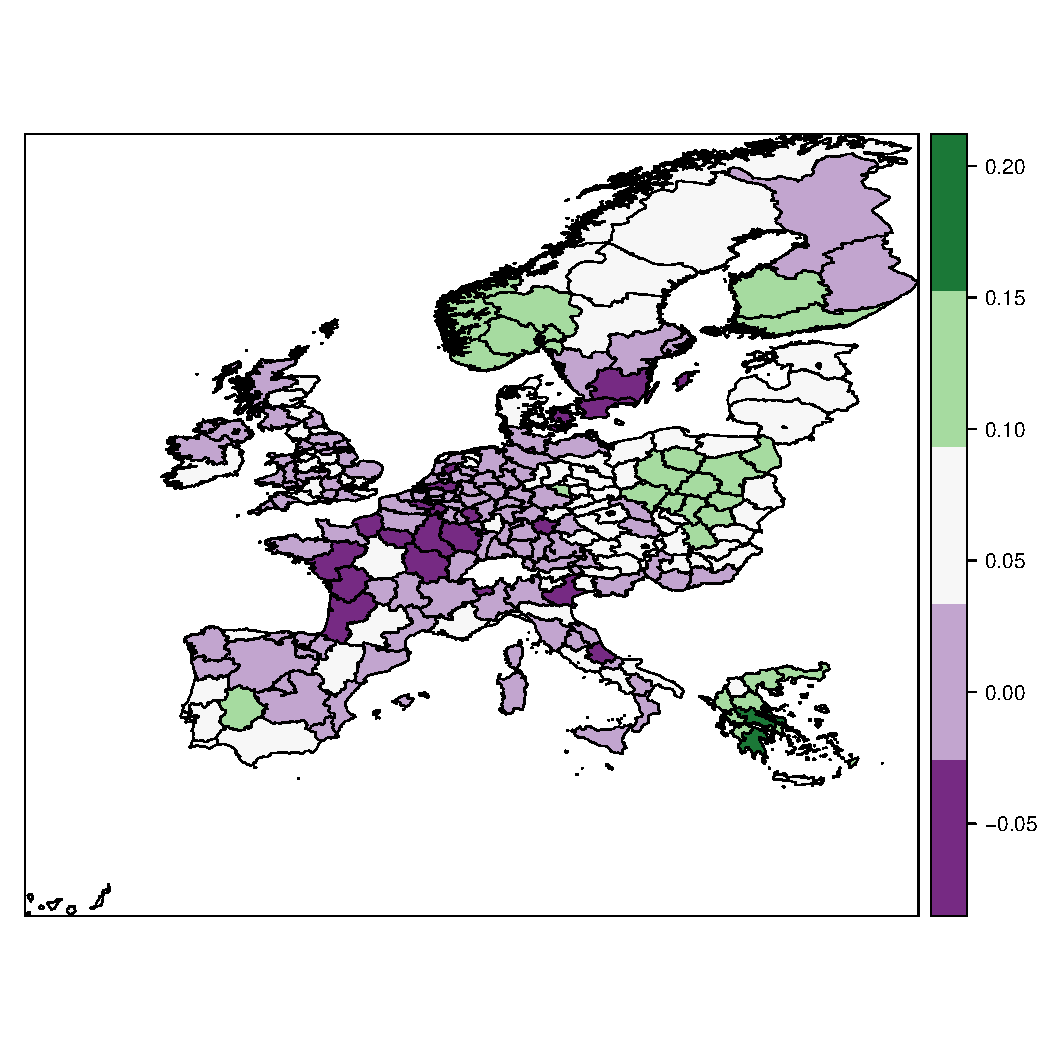
\includegraphics[width=0.8\textwidth]{fig/TEfrontierdiff}
	\caption{Difference frontier vs. SEM frontier model for energy and manufacturing.}
	\label{fig:TEfrontierdiff}
\end{figure}

Figure \ref{fig:TEfrontierdiff} shows the difference between the non-spatial technical efficiencies and the efficiencies, which are generated by a SEM frontier model. Clearly, the introduction of spatial dependence ensures that regions in the center become less efficient and regions in the periphery become more efficient (the distribution of technical efficiencies over regions becomes more homogeneous). In other words, regions in the periphery produce technically inefficient but less so when taking their relative geographical location into account. Thus, where regions are located matters just as their economic structure. 
 
I continue with the SEM frontier model and turn to sectoral estimations in Table \ref{tab:resultssectors}, where I specify for each sector a SEM frontier model.\footnote{Checks with other specifications show that the SEM frontier model always performs best in terms of log-likelihood.}
%
\begin{table}[h]
\small
\centering
\renewcommand\arraystretch{1.3}
\def\onepc{$^{\ast\ast}$} \def\fivepc{$^{\ast}$}
\def\tenpc{$^{\dag}$}
\def\legend{\multicolumn{11}{l}{\footnotesize{Significance levels
			:\hspace{1em} $\dag$ : 10\% \hspace{1em}
			$\ast$ : 5\% \hspace{1em} $\ast\ast$ : 1\% \normalsize}}}
		\caption{Estimation of SEM frontier models for separate sectors ($N=256$ and standard errors between parentheses)}
		\label{tab:resultssectors}
\begin{tabular*}{\columnwidth}{@{\extracolsep{\fill}} l D{.}{.}{2.5}@{} D{.}{.}{2.5}@{} D{.}{.}{2.5}@{} D{.}{.}{3.5}@{} D{.}{.}{3.5}@{} D{.}{.}{3.5}@{} }
	\toprule
	& \multicolumn{1}{c}{Agric.} & \multicolumn{1}{c}{E \& M} & \multicolumn{1}{c}{Constr.} & \multicolumn{1}{c}{Distri.} & \multicolumn{1}{c}{Serv.} & \multicolumn{1}{c}{NM. Serv} \\
	\midrule
	Constant          & 2.43^{***} & 4.03^{***}  & 2.11^{***}  & 1.24^{***}  & 2.05^{***} & 1.74^{***}  \\
	& (0.71)     & (0.25)      & (0.22)      & (0.17)      & (0.29)     & (0.19)      \\
	$\ln$(Capital)    & 0.68^{***} & 0.58^{***}  & 0.61^{***}  & 0.69^{***}  & 0.71^{***} & 0.61^{***}  \\
	& (0.03)     & (0.03)      & (0.04)      & (0.03)      & (0.03)     & (0.03)      \\
	$\ln$(Employment) & 0.21^{***} & 0.44^{***}  & 0.39^{***}  & 0.30^{***}  & 0.29^{***} & 0.39^{***}  \\
	& (0.03)     & (0.03)      & (0.04)      & (0.04)      & (0.03)     & (0.04)      \\
	$\sigma$          & 0.26^{***} & 0.29^{***}  & 0.28^{***}  & 0.24^{***}  & 0.17^{***} & 0.25^{***}  \\
	& (0.01)     & (0.02)      & (0.02)      & (0.02)      & (0.01)     & (0.02)      \\
	$\alpha$          & -0.03      & -1.41^{***} & -1.19^{***} & -1.54^{***} & -0.02      & -1.68^{***} \\
	& (1.44)     & (0.37)      & (0.29)      & (0.34)      & (0.75)     & (0.32)      \\
	$\lambda$         & 0.57^{***} & 0.78^{***}  & 0.76^{***}  & 0.78^{***}  & 0.59^{***} & 0.81^{***}  \\
	& (0.08)     & (0.09)      & (0.08)      & (0.08)      & (0.08)     & (0.08)      \\
	\midrule
	Log Lik.          & 62.92      & 94.86       & 94.19       & 149.78      & 164.88     & 143.52      \\
	\bottomrule
\end{tabular*}
\end{table}
%
Note again that all output elasticities point to constant returns to scale. Energy and manufacturing seems to be the most capital intensive sector and non-market services the most labour intensive sector. The most skewed sectors, with $\alpha$'s around $-1.6$, and thus the sectors with the largest differences in regional efficiency are distribution and non-market services. Spatial dependence is in allmost all sectors---except perhaps agriculture and services---high with $\lambda$'s close to 0.8.

Figure \ref{fig:sectoralsfe} shows the maps of the estimated regional technical
efficiencies provided by the estimates in Table \ref{tab:resultssectors}.
Obviously, there are large differences in the regional distribution of technical
efficiencies, but on average regions in the center of Europe seem to have larger
technical efficiencies than regions in the periphery. Moreover, agriculture has
on average a much more homogeneous regional technical efficiency than, e.g.,
construction or distribution, where regional differences are much more pronounced. 

\begin{figure}[ht!]

\subfloat[Agriculture]{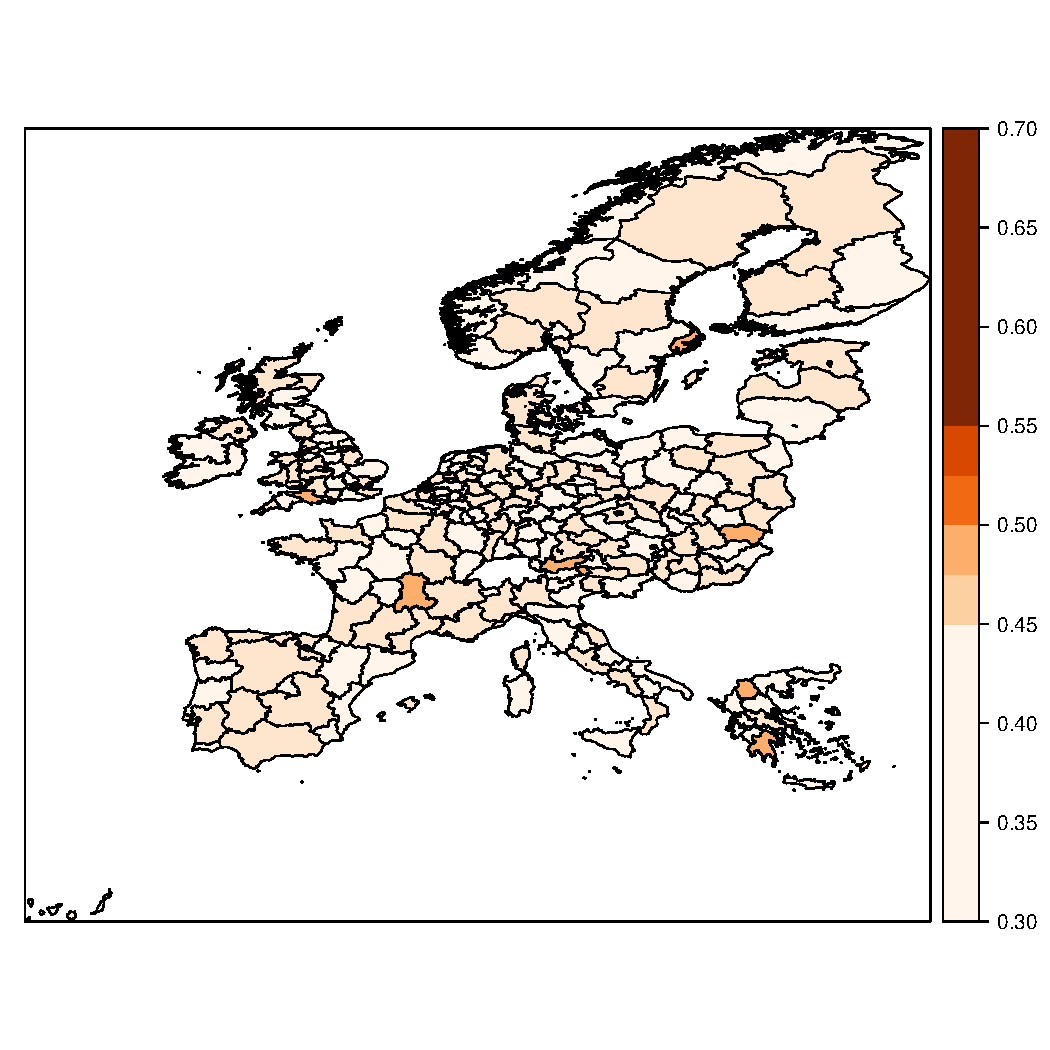
\includegraphics[width = 0.45\textwidth]{fig/TEfrontierAgr}}
\subfloat[Energy \& manufacturing]{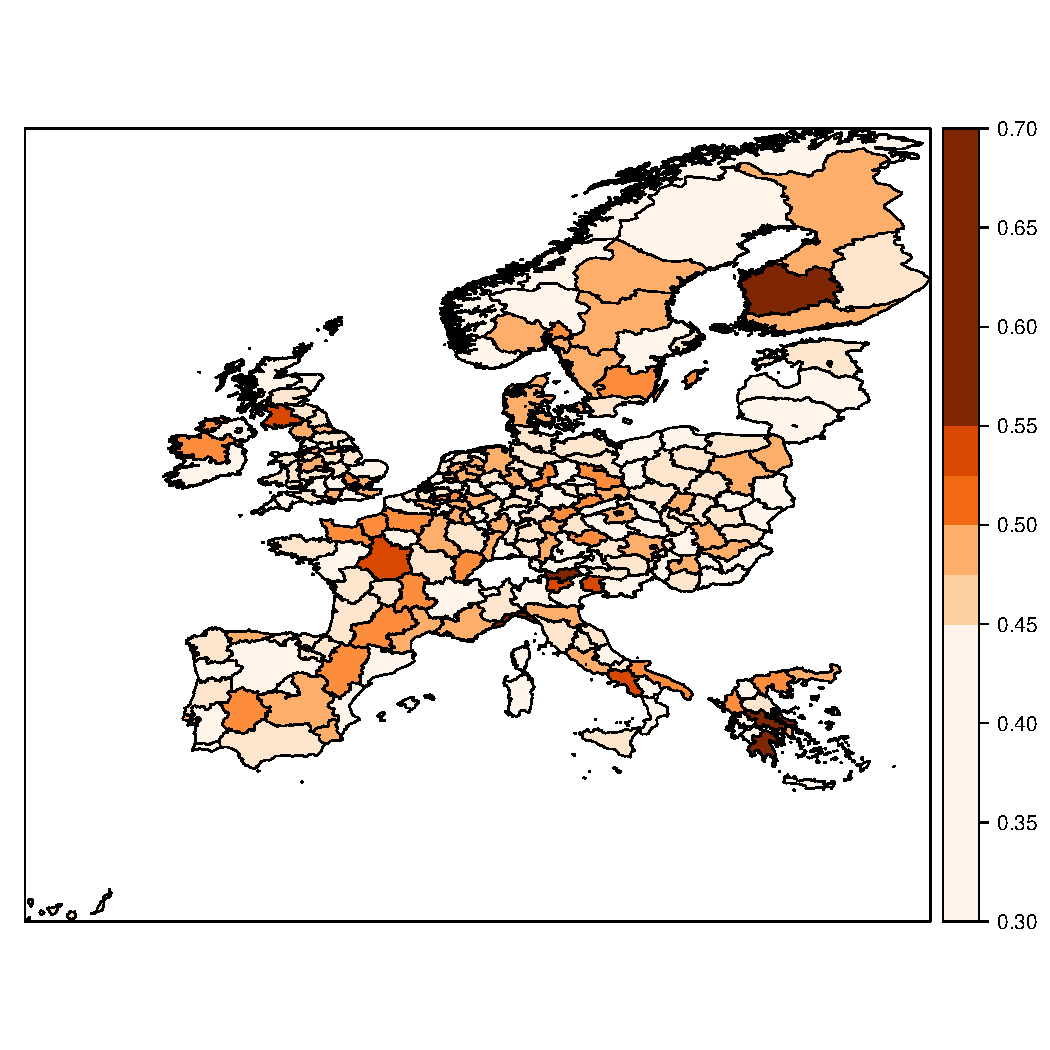
\includegraphics[width = 0.45\textwidth]{fig/TEfrontierEM}}\\[-5ex]
\subfloat[Construction]{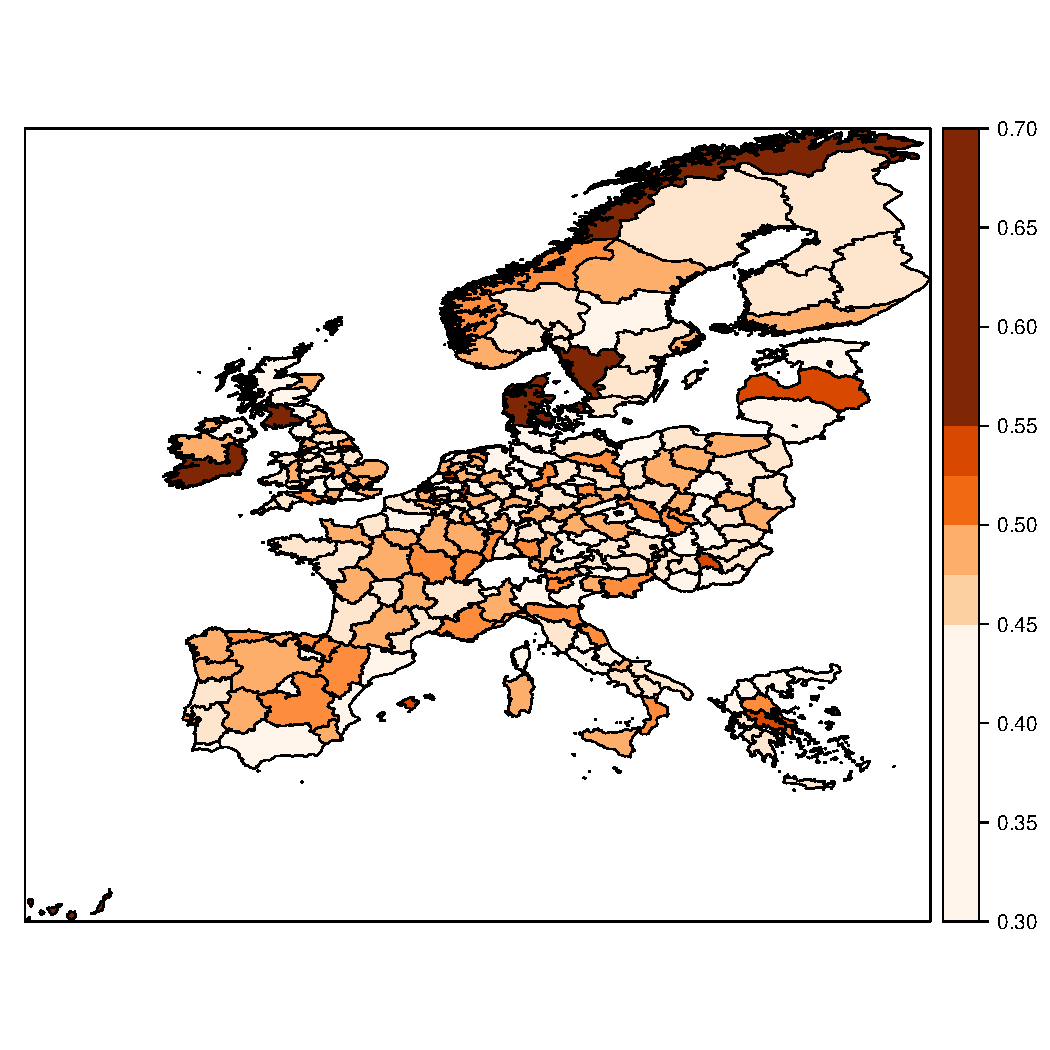
\includegraphics[width = 0.45\textwidth]{fig/TEfrontierCon}}
\subfloat[Distribution]{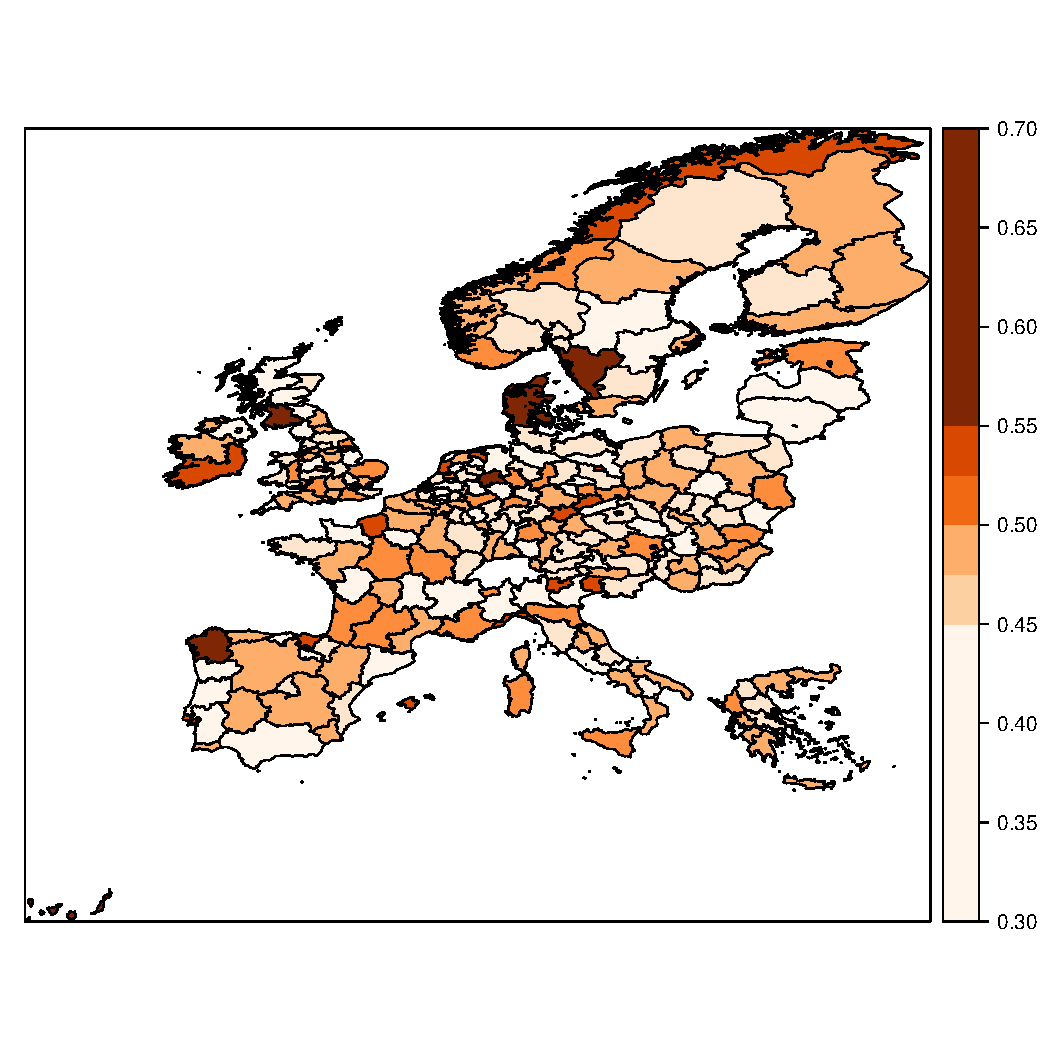
\includegraphics[width = 0.45\textwidth]{fig/TEfrontierDist}}\\[-5ex]
\subfloat[Services]{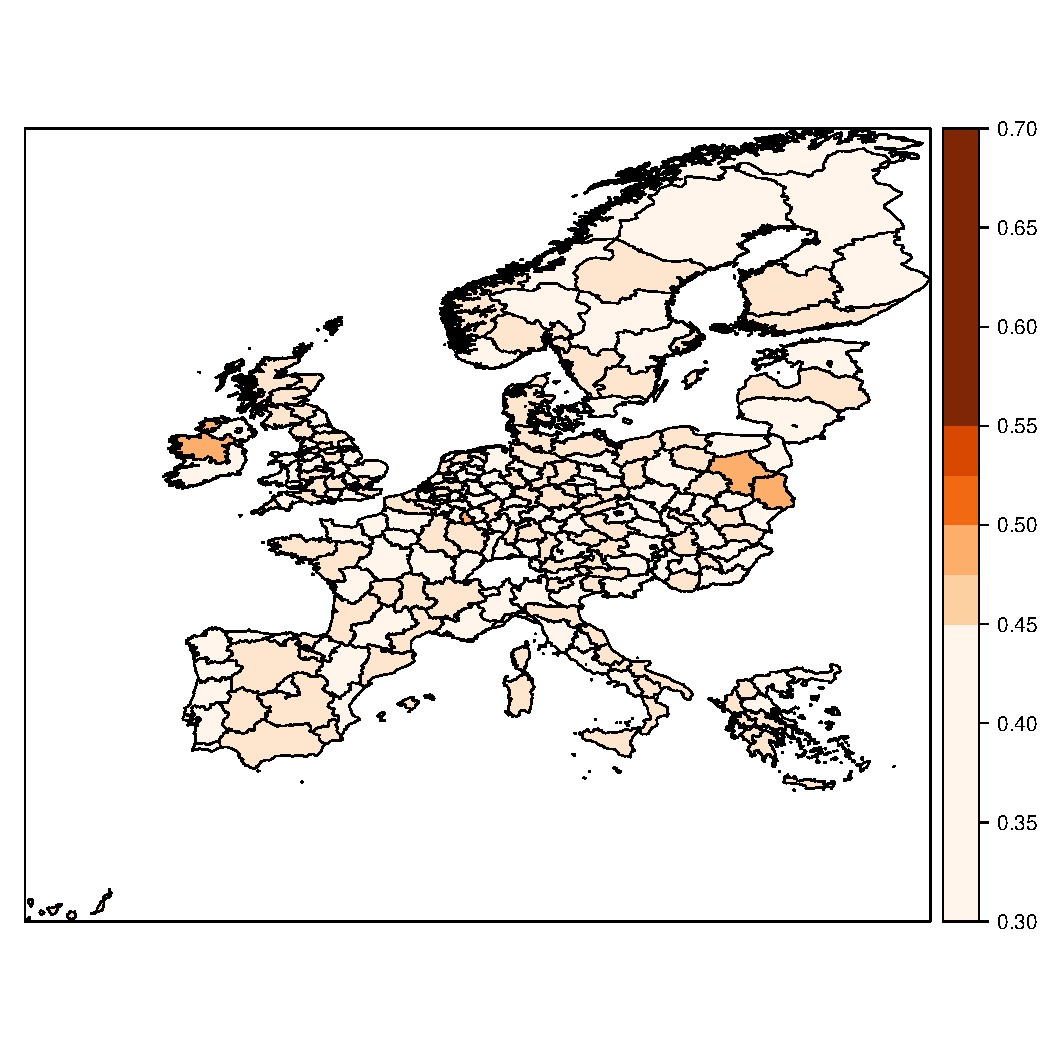
\includegraphics[width = 0.45\textwidth]{fig/TEfrontierServ}}
\subfloat[Non-market services]{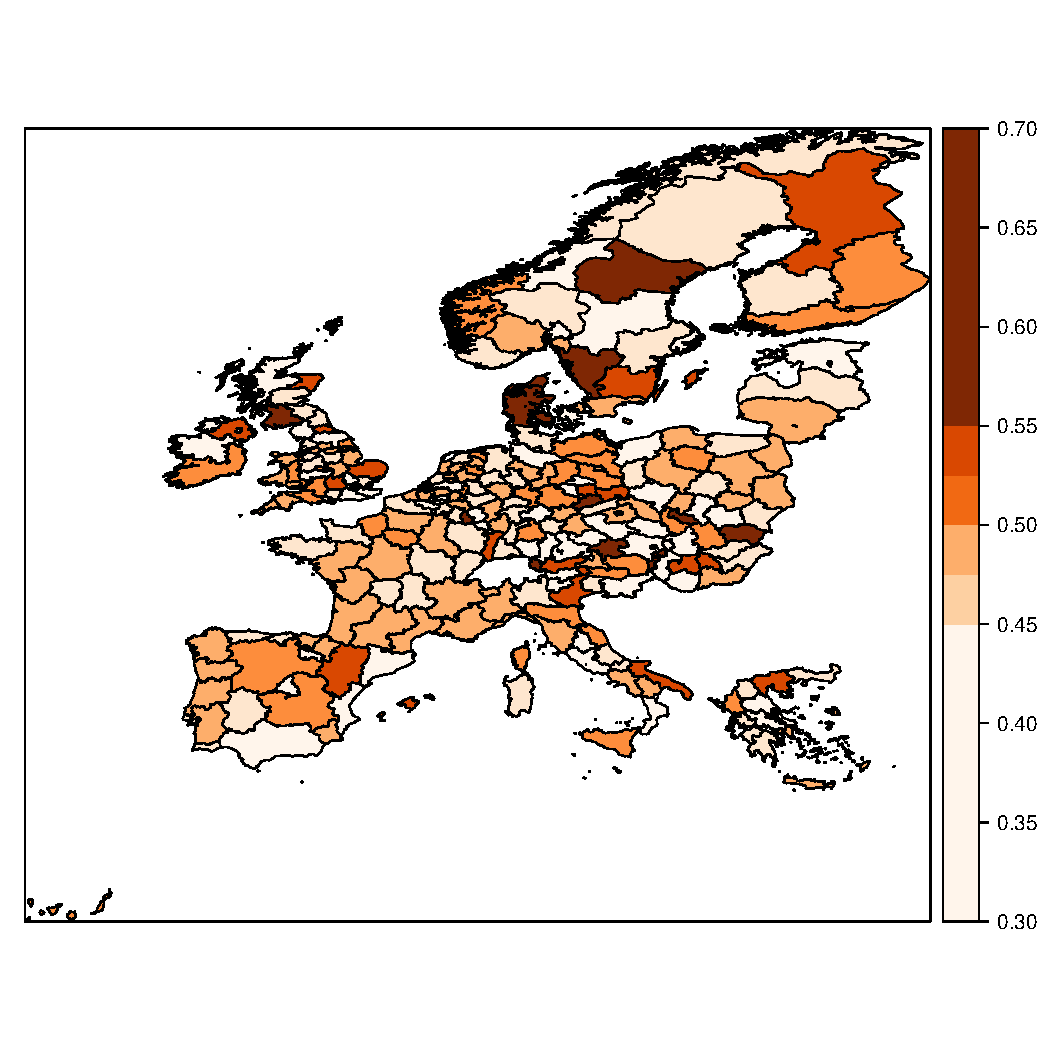
\includegraphics[width = 0.45\textwidth]{fig/TEfrontierNMServ}}
\caption{Technical efficiencies across Europe for 6 sectors}
\label{fig:sectoralsfe}
\end{figure}
%
\section{In conclusion}
%
The main aim of this paper was to introduce spatial dependence in stochastic production frontier analysis. I did this by adopting a multi-variate skew-normal distribution function approach, which I argue is (\emph{i}) straightforward to estimate, (\emph{ii}) able to separate spatial dependence in the error term and technical efficiencies, and (\emph{iii}) produce consistent estimates. 

Obviously, there is more to this because technical efficiencies may be spatially
depend as well or there might be a general spatial lag process present. For
instance, there are spillovers in the adoption of new technology that improve
the efficiency or there are specific institutions, such as former guilds or
unions, that prohibit the adoption of new technologies are spatially
concentrated. However, when looking at the efficiency of regions, taking into
account spatial dependence---whether in the inefficiency part or not---strongly
improves the estimates of the technical efficiencies; in other words, they
become less biased. However, estimating combinations of multivariate normal and
multivariate truncated normal distributions require more complex estimation
methods, whether in the form of simulation estimation methods or expectation-maximization (EM) type of algorithms.

When looking at European regions, taking spatial dependence into account
controls to a certain extent for the core-periphery pattern in Europe. Thus,
regions in the periphery do not produce that inefficiently only because of their
economic structure, but partly as well because of their location and the related
diminished access to knowledge and information. Obviously, these estimations are
restrictive regarding the data and specification I use. But for illustration
purposes they fit perfectly and point to the fact that peripheral regions are
performing partly worse because of their remote location and decreased access to
all sorts of networks.
%
\begin{spacing}{1.2}
	\printbibliography
\end{spacing}

\end{document}
